\documentclass[12pt,a4paper]{article}
\usepackage{rmpackages}																% usual packages
\usepackage{rmtemplate}																% graphic charter
\usepackage{rmexocptce}																% for DS with cptce eval

\usepackage{fontawesome}
\newcommand{\thumbsup}{\marginpar{\faThumbsOUp}}

%\cfoot{} 													% if no page number is needed
%\renewcommand\arraystretch{1.5}		% stretch table line height

\newcommand{\ritem}{\refstepcounter{enumi}\item[\writeit{} \theenumi .]}

\begin{document}

\begin{header}
TP -- La plume et le marteau
\end{header}

\begin{multicols}{2}
\begin{center}
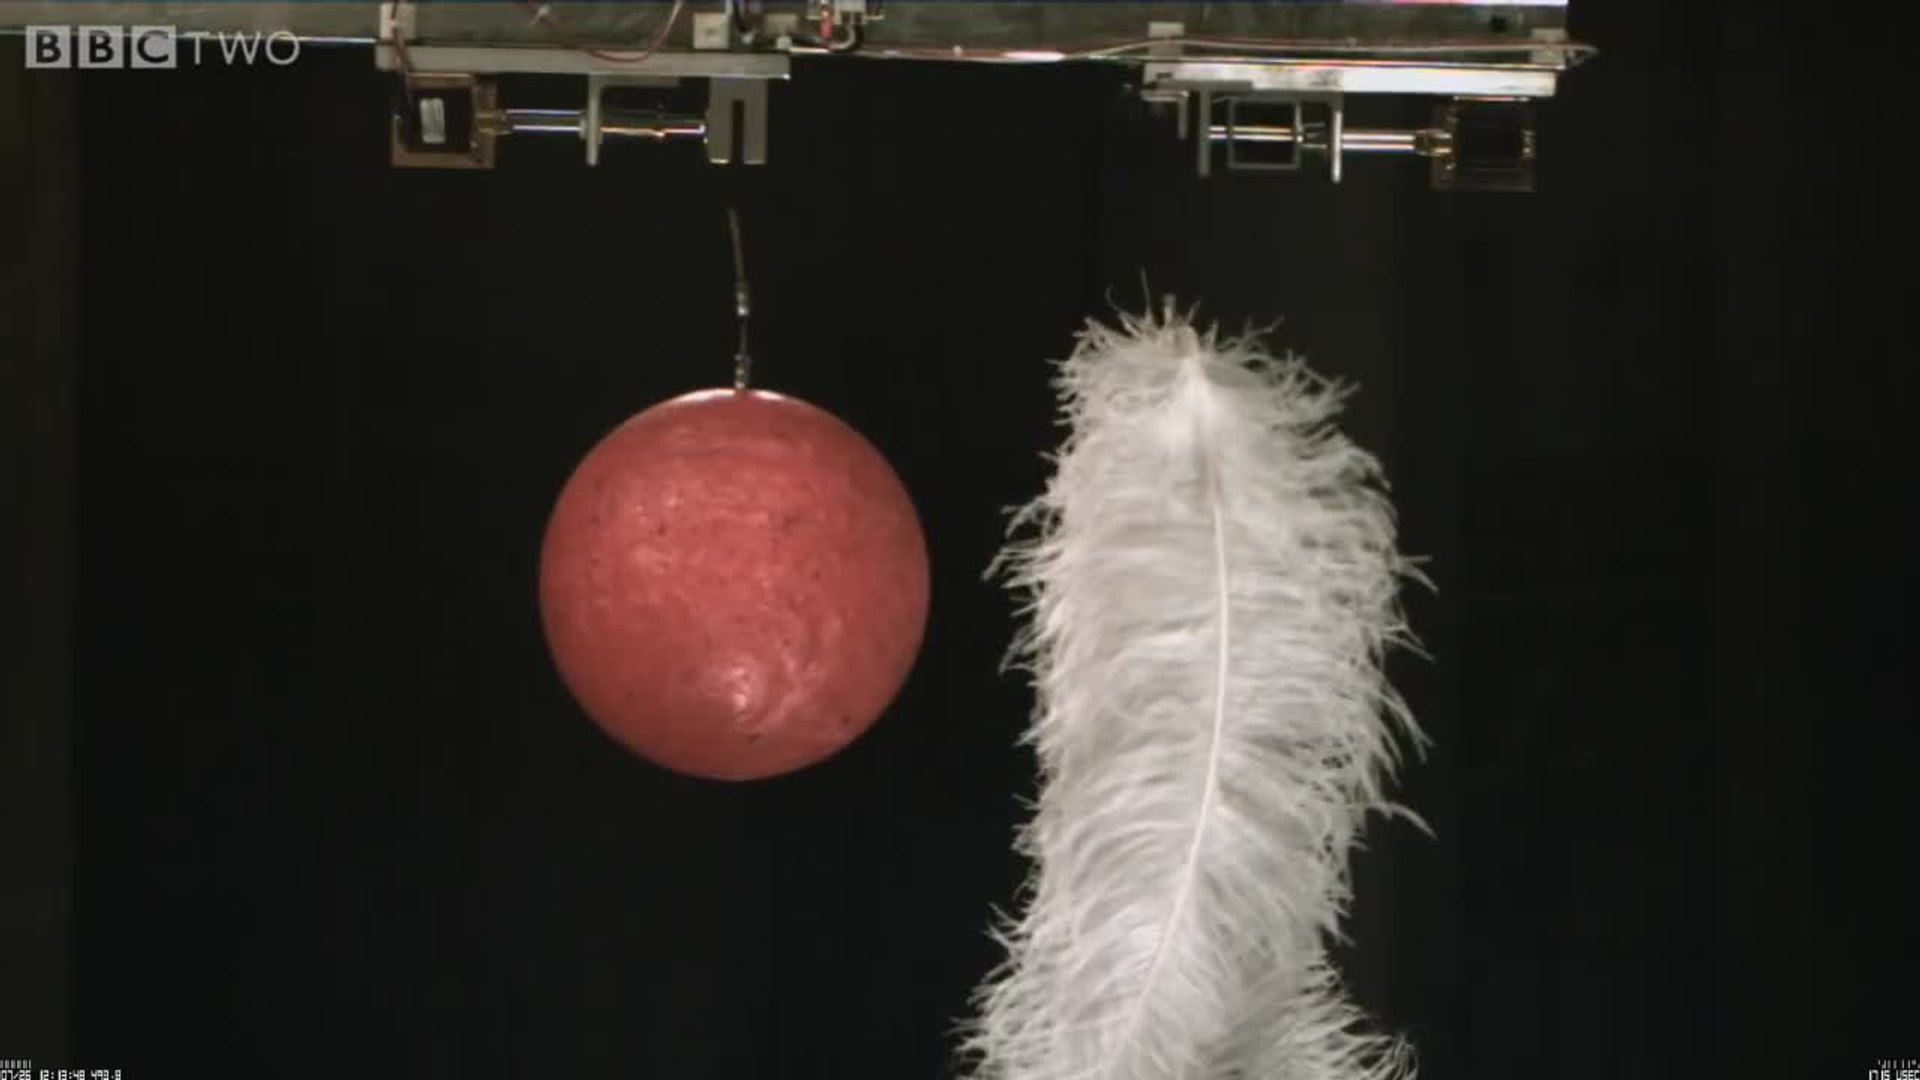
\includegraphics[width=\linewidth]{images/plumarteau.jpg}
\end{center}

En 1971, les astronautes de la mission Apollo 15 se posent sur la Lune.
David Scott, leur commandant, en profite pour vérifier l'hypothèse de Galilée sur la chute des corps formulée au XVII\textsuperscript{ème} siècle.

Depuis, les scientifiques de la NASA ont reproduit cette expérience sur Terre dans une chambre à vide géante de laquelle ils ont presque entièrement retiré l'air.
\end{multicols}

\section*{L'expérience}

\begin{enumerate}
\item \rea{} Copier-coller tout le dossier \og TP Plume 2 \fg{} dans votre espace de travail personnel (Ordinateur \textrightarrow{} Ma classe \textrightarrow{} Documents en consultation \textrightarrow{} Physique-Chimie) 

\item Regarder la vidéo de l'expérience originale (\texttt{vidéo1} à partir de 0'58'') puis celle réalisée sur Terre (\texttt{vidéo2}).
Vous pourrez retrouver ces vidéos ici \href{https://youtu.be/oYEgdZ3iEKA}{https://youtu.be/oYEgdZ3iEKA} et là \href{https://youtu.be/Ha0b8n5puJM}{https://youtu.be/Ha0b8n5puJM}.
\end{enumerate}

\section*{Quel modèle choisir ?}

On s'intéresse à la deuxième expérience et on souhaite tout d'abord représenter les positions successives d'une plume (modélisée par un point) au cours de sa chute.

\begin{enumerate}[resume]
\ritem \app{} \anarai{} Identifier le système étudié et indiquer le référentiel choisi dans la vidéo pour étudier le mouvement de la plume.

\ritem \rco{} Décrire le mouvement d'une plume dans ce référentiel (trajectoire et vitesse).
\label{quest:trajectoire}
\end{enumerate}

Le tableau ci-dessous indique la distance entre le point de départ et la plume en fonction du temps.

\begin{center}
\begin{tabular}{|lc|c|c|c|c|c|c|c|}
\hline
\textbf{Temps} & (s) & 0{,}00 &  0{,}45 &  0{,}90 &  1{,}35 &  1{,}80 &  2{,}25 &  2{,}70 \\
\hline
\textbf{Distance} & (m) & 0{,}00 & 0{,}97 & 3{,}89 & 8{,}75 & 15{,}56 & 24{,}31 & 35{,}00 \\
\hline
\end{tabular}
\end{center}

\begin{enumerate}[resume]
\item \rea{} Ouvrir le programme \texttt{chute\_libre.py} et l'exécuter 
\includegraphics[height=0.75\baselineskip]{images/edupython_execute.png}.

\ritem \app{} À quoi correspondent les tableaux \texttt{t}, \text{X} et \texttt{Y} des lignes 7 à 9 ?
\thumbsup
\end{enumerate}

\begin{appel}
\app{}
\end{appel}

\begin{enumerate}[resume]
\ritem \app{} Quelle ligne permet de représenter les positions successives de la \textbf{plume} ?

\ritem \rea{} Calculer la vitesse moyenne de la plume pendant toute sa chute. \thumbsup
\end{enumerate}

\section*{Vecteur vitesse}

\begin{enumerate}[resume]
\ritem \rea{} Donner les caractéristiques du vecteur vitesse $\vec{v_5}$ au point $M_5$.
\label{quest:carac_vitesse}
\end{enumerate}

\begin{appel}
\rea{} 
\end{appel}

\begin{enumerate}[resume]
\ritem \app{} \anarai{} Supprimer le \# de la ligne 33 et exécuter le programme.
Décrire les changements observés sur le graphe.

\ritem \anarai{} \val{} À quoi correspondent les valeurs \texttt{x}, \texttt{y}, \texttt{vx} et \texttt{vy} des lignes 27, 28, 30 et 31 ?
\thumbsup
Justifier.

\ritem \rea{} \val{} En vous aidant de la question~\ref{quest:carac_vitesse}, modifier les valeurs \texttt{x}, \texttt{y}, \texttt{vx} et \texttt{vy} pour représenter le vecteur vitesse $\vec{v_5}$.
\end{enumerate}

\begin{appel}
\val{}
\end{appel}

\newpage{}

\section*{Supplément 1 (2)}

\begin{enumerate}[resume]
\item \rea{} En vous aidant des lignes 27 à 33, modifier le programme pour représenter également le vecteur vitesse $\vec{v_1}$ au point $M_1$. \thumbsup
\textit{Votre programme ne devra contenir aucune valeur numérique.}

\ritem \app{} \val{} Commenter l'évolution des caractéristiques du vecteur vitesse au cours du mouvement.
Est-ce cohérent avec la question \ref{quest:trajectoire} ? Justifier.
\end{enumerate}

\begin{appel}
\end{appel}

\section*{Supplément 2 (2)}

\begin{enumerate}[resume]
\item \anarai{} \rea{} En vous aidant du programme \texttt{chute\_libre.py}, compléter le programme \texttt{saut.py} pour représenter le vecteur vitesse au point $M_4$. \thumbsup
\end{enumerate}

\begin{appel}
\end{appel}

\end{document}